\chapter{Chapter 3: The functional organization of phonemes in the STG}

\section{Introduction}
A long lasting controversy persists in psycholinguistic research regarding the involvement of the motor system in speech perception. The motor theory of speech perception \citep{liberman1967perception, liberman1985motor} describes phoneme perception in terms of the articulatory gestures that generate it. According to this theory, the objects of speech perception are the intended phonetic gestures of the speaker, such as, ‘lip rounding’, or ‘jaw raising’. For example, the phoneme [m] consists of a labial stop gesture combined with a velum-lowering gesture. As an alternative view, auditory theories argue that phonetic processing depends directly on properties of the auditory system \citep{jakobson1951preliminaries, stevens1972quantal, stevens1989quantal, stevens2002toward}. According to this view, listeners identify spectrotemporal patterns in phoneme waveforms and match them with stored acoustic representations. For example, vowels are characterized by a roughly bimodal spectra and sibilant fricatives by high-frequency energy.

The motor theory arose from an early observation that phoneme percepts are invariant across different contexts \citep{cooper1952some, liberman1967perception}. In the case of coarticulation, several gestures overlap in time, which may cause the acoustic waveform of the same intended gesture to be significantly different than when it is pronounced in isolation. Therefore, a particular gesture can be represented by different acoustic waveforms in different phonetic contexts. Additional variation exists in the acoustic signal due to inter-speaker variability.  This considerable variability led the supporters of the motor theory to propose that the objects of speech perception are not to be found in acoustics.

Phoneme perception has been the focus of many neuroimaging studies \citep{liebenthal2005neural, dehaene2005neural, mottonen2006perceiving, desai2008left, liebenthal2010specialization,  formisano2008saying, binder2000human, Dewitt2012}. One common method in these studies uses sophisticated baselines to speech, such as rotated speech, to elicit activation in regions that are selective to speech, but not to nonphonemic contrasts. The results describe a complex picture of hierarchically-organized phoneme processing in the temporal lobe, from primary auditory and early posterior auditory areas to higher-level processing in the anterior, ventral Superior Temporal Gyrus (STG) and Superior Temporal Sulcus (STS). 

Invasive electrophysiological recordings in humans provide a precious glimpse into the neural representations of linguistic entities, such as the objects of speech perception, with high temporal resolution and spatial localization compared to non-invasive recording techniques. Invasive techniques can record extracellular electrical activity either at the level of local field potentials (LFPs), or at the level of action potentials generated by single cells. Various types of electrodes are commonly used, such as, subdural grids \citep{viventi2011flexible}, depth electrodes \citep{fried1999cerebral}, Utha array \citep{nordhausen1996single}, or microdialysis \citep{fried2001increased}.

Recent electrocorticography (ECoG) studies, using subdural grids, have contributed to our understanding of neural encoding in higher-level auditory cortex, and shed new light on the long-lasting debate in speech perception. \citet{pasley2012reconstructing} showed that speech waveforms can be reconstructed from neural activity in the lateral STG, suggesting that encoded information in this region is mainly acoustic. More recently, \citet{Mesgarani2014} characterized the functional organization of phonemes in the peri-Sylvian speech cortex. This study provides a detailed examination of neural representations of phonemes in the STG of human subjects during listening to natural speech. Examining the functional organization in this region, they found that phoneme representations cluster according to acoustic features in an hierarchical manner. Remarkably, the dominant organizing acoustic features are the same distinctive features defined by linguists half a century ago \citep{ChomskyHalle1968}, such as, sonority, nasality and stridency. Moreover, an order was found among features: manner-of-articulation features produce a neural invariance that is more prominent than that related to place-of-articulation - neural representations are clustered according to manner-of-articulation features, whereas neural responses to the the same place-of-articulation feature can vary considerably. More recently, a similar order was found also using EEG recordings \citep{khalighinejad2017dynamic}. This order is consistent with early observations from language acquisition. During language development, manner-of-articulation distinctions are acquired early during childhood, compared to the place-of-articulation ones \citep{jakobson1968child, grodzinsky2014neural}. Taken together, these findings support the auditory view of speech perception rather than motor theories. Other ECoG studies \citep{bouchard2013functional, cheung2016auditory}, further examined the functional organization of phonemes outside the STG and tested its dependency on the experimental task (listening vs. production). Results show that the organization can significantly differ across brain regions and tasks: \citet{bouchard2013functional} showed that the functional organization of phonemes in the vSMC during production is dominated by place-of-articulation features (e.g., labial, alveolar, velar and glottal), in contrast to manner-of-articulation features in the STG during listening. More recently, the functional organization in the same region was found to differ also across tasks. Whereas during phoneme production, the dominant organizing feature of neural activity in the vSMC is place-of-articulation, during listening, the organization in the same region was found to be dominated by manner features, similarly to the STG \citep{cheung2016auditory}.

ECoG studies have greatly enriched our understanding of the neural basis of speech perception.  However, the electrical activity recorded in ECoG grids reflects average responses of large neuronal populations, as non-invasive methods, and is therefore limited in providing insights into activity patterns of single cells. Describing and construing single-cells activity is indispensable for a complete theory of the neural basis of speech perception, and cognitive processes in general. Single-unit recording was pioneered at the mid of the previous century, and was later developed to obtain multiple single-unit recordings from deep brain structures in humans \citep{fried1999cerebral} (for a review, \citealp{engel2005invasive, mukamel2012human, cash2015emergence}). It provides unique spatiotemporal resolution and valuable information about processes that are unique to humans, such as language \citep{heit1988neural, creutzfeldt1989neuronal, tankus2012structured, ossmy2015decoding}.

Consistent with findings from ECoG and EEG studies, single-cell studies on phonetic processing revealed a multidimensional neural representation of phonemes by demonstrating that STG neurons are tuned to subsets of phonemes and have a sparse coding scheme \citep{creutzfeldt1989neuronal, chan2013speech}. However, the functional organization of phonemes at the cellular level is still poorly understood. Specifically, whether single STG neurons encode phonemes in an hierarchical way, as was revealed by analyzing gamma activity in ECoG studies, with larger invariance to manner- compared to place-of-articulation features.

This study addressed three questions regarding spiking activity of STG neurons in response to phonemic stimuli. First, we examined whether neural response of STG units is selective to specific phonemes, or whether phoneme stimuli are distributively represented across population activity. Second, we examined whether the functional organization of phonemes as revealed by single-cells activity is dominated by manner- or by the place-of-articulation dimension. Manner features can be mapped to acoustic properties, therefore providing support to auditory theories of speech perception, whereas place features can be mapped to motor gestures, thus providing support to the motor theory of speech perception. Finally, we examined whether the functional organization of phonemes as revealed by single-cells activity matches with that of the cognitive one. We made use of the same set of stimuli in both a behavioral experiment with normal subject and in the experiment with neurosurgical patients implanted with depth electrodes.

\begin{figure}[H]
\vspace{.3in}
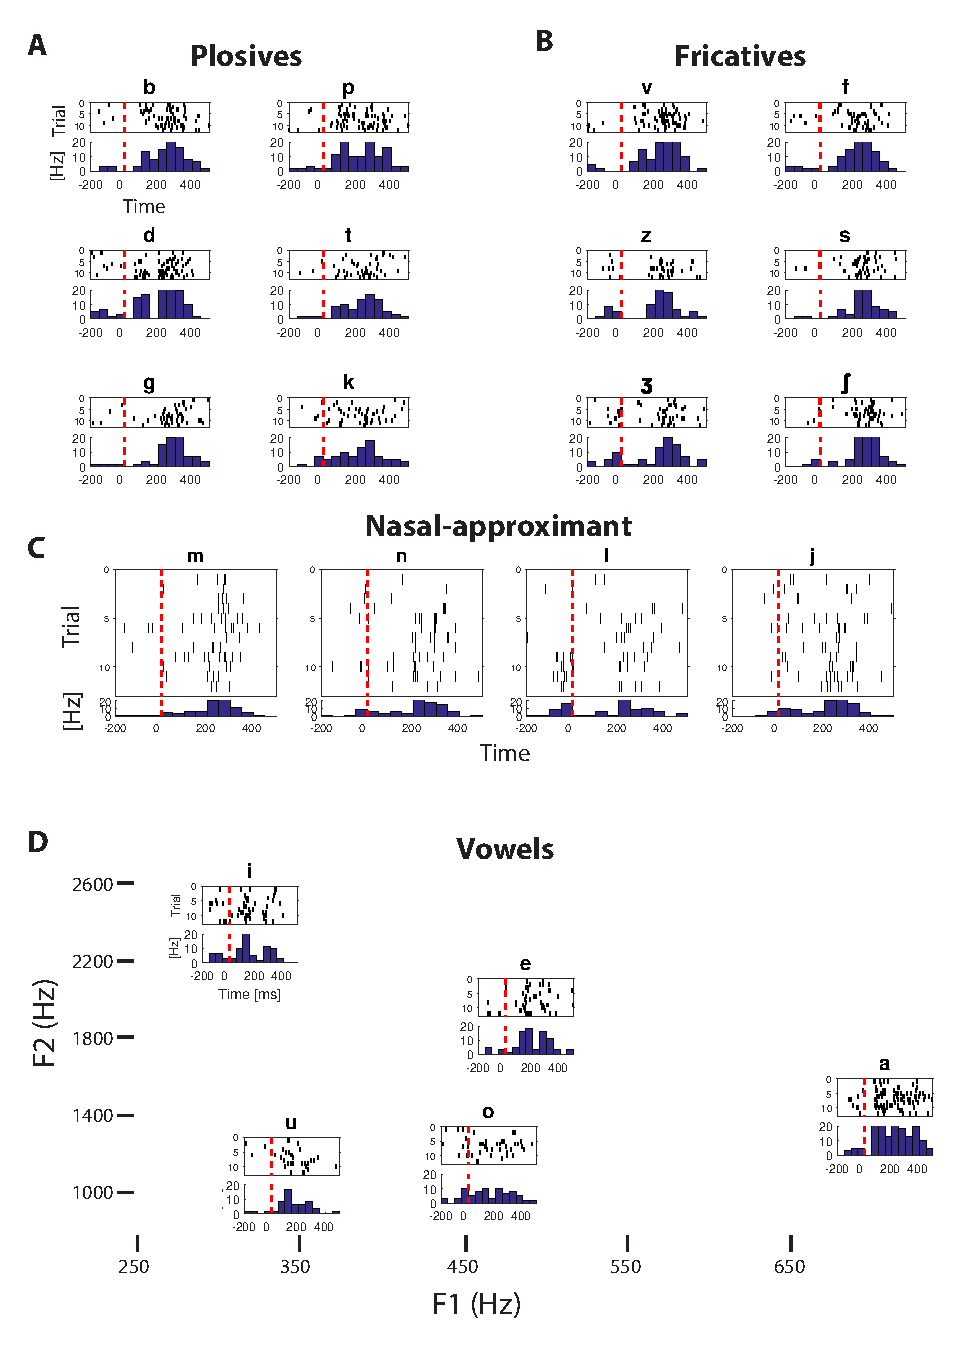
\includegraphics[width=\linewidth]{Figures/Ch3/Figure2_new.eps}
\caption{Raster and PSTH plots for an example unit, from one of the patients. (A) Voiced (left) and unvoiced (right) plosives (B) voiced (left) and unvoiced (right) fricatives (C)  nasal-approximant (left) and affricate (right) phoneme (D) Vowel rasters are embedded in approximant locations in the formant space.}
\end{figure}

\section{Results}
To address the questions of this study, we recorded neural activity from six patients, implanted with intracranial depth electrodes, during a listening task in which auditory stimuli of various phonemes were presented (\textit{methods}, section 3.3.1 and 3.3.3). Each of the following subsections addresses a research question of this chapter: section 3.2.1 presents and characterizes spiking activity in the STG in response to phoneme stimuli. Section 3.2.2 examines whether the functional organization is more dominated by place-of-articulation or by manner-of-articulation features. Finally, section 3.2.3 compares the similarity structure of phoneme representations as revealed by population spiking activity and that derived from a behavioral experiment, using the same set of stimuli in both experiments.

\subsection{Basic characteristics of the neural responses}
We present examples of spiking activity of STG units in response to phonemic stimuli, and characterize the population activity with basic measures. Units were sorted using WaveClus and assessed for responsiveness to phoneme stimuli (\textit{methods}, section 3.3.3). Figure 3.1 presents an example of raster and Peri-Stimulus Time Histograms (PSTH) plots from one STG unit from one patient. Consonants are grouped according to plosives, fricatives and nasal-approximant (Panels A-C); Vowels are embedded in approximant locations in formant space (Panel D). 

Reviewing the various response profiles to consonant phonemes, some profiles seem to contain two activity peaks (see, e.g., in the PSTHs of /bpds/). This dual-mode response may be, at part, due to the structure of the stimuli, which contain a consonant followed by a vowel (among other possible factors, such as excitation-inhibition cycle, or neuronal fatigue). Since the vowel in the CV syllables is always /a/, it suggests that the time period for which the response is most informative about consonant identity may be around the early peak. We therefore first identify, for each unit, the time period for which the neural response is most informative about the first phoneme identity.

\begin{figure}
\vspace{.3in}
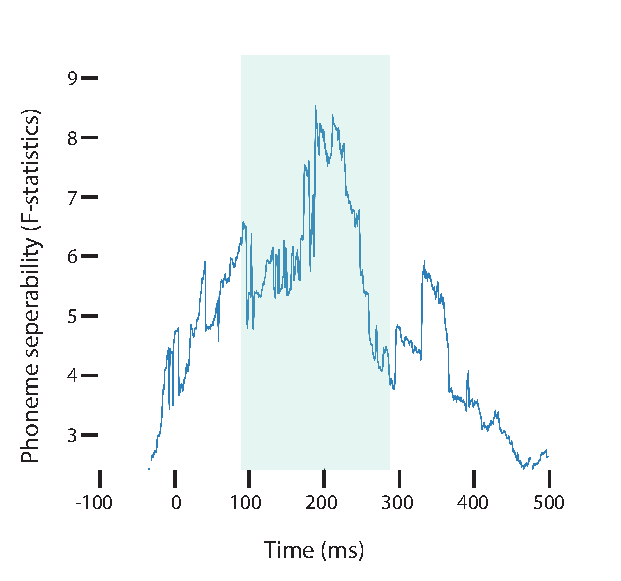
\includegraphics[width=\linewidth, height=7cm]{Figures/Ch3/Figure1_new.eps}
\caption{Optimal time window: results for the between-phoneme to within-phoneme variability ratio of the spike-count (F-statistic), for a running window of 200ms (calculated between 0-500ms), averaged across units. Time values represent the center of the time window. Optimal integration window (shaded area) is determined according to the peak.}
\end{figure}

To this end, we define an optimal time window as one for which the neural responses to the different phonemes are most separable. As a measure for separability we estimate the between-phoneme to within-phoneme variability ratio (F-statistic) of the spike-counts. We calculate this measure for various time windows and identify the one for which it is maximal. Figure 3.2 shows the average F-statistic across all units, for a running time window of 200ms duration. The size of the time window was chosen similar to previous single-cell studies (e.g., \citealp{chan2013speech}); window sizes in the range 100-300ms did not have a substantial effect on the results. Figure 3.2 shows that the center of the most informative time window peaks, on average, around 200ms after stimulus onset. This time period is similar to ERP studies showing that the difference between phonemic and nonphonemic processes peaks at approximately 200ms \citep{liebenthal2010specialization}.

\begin{figure}[H]
\vspace{.3in}
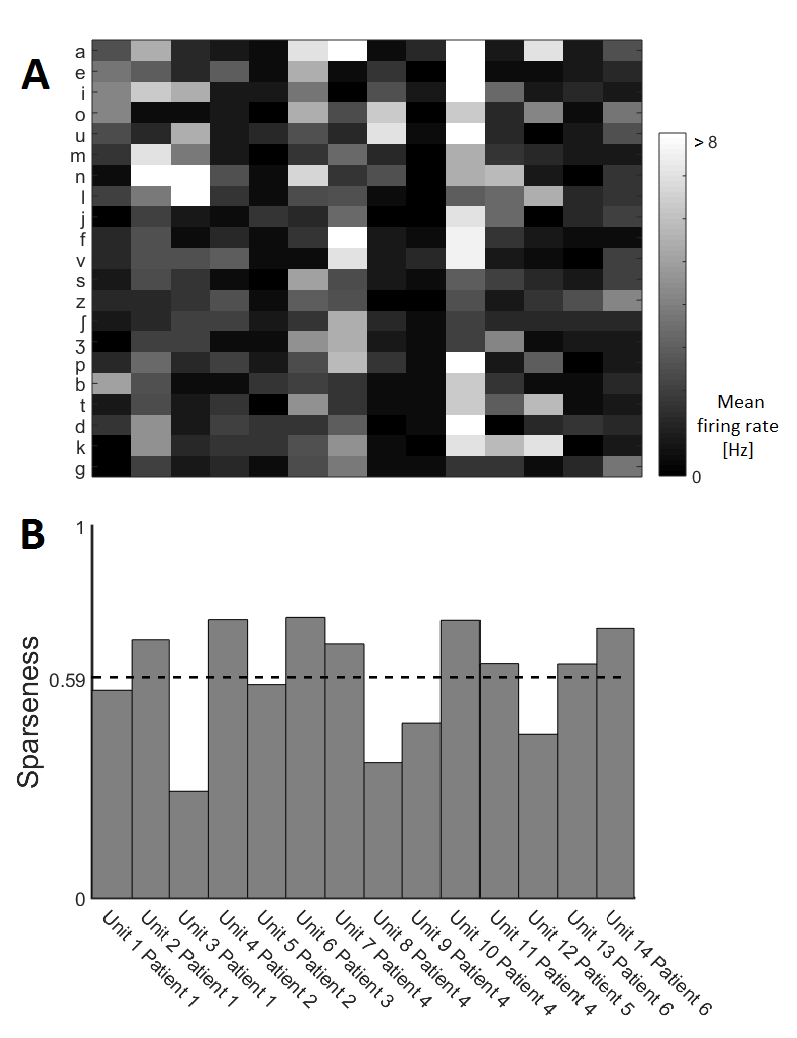
\includegraphics[width=\linewidth]{Figures/Ch3/ch3_fig3.png}
\caption{(A) Mean firing rates for all units in response to all phoneme stimuli. Color scale represents mean firing-rates calculated in the optimal time window; (B) Sparseness of neural responses for all units. Dashed line represents mean sparseness across all units ($\bar{a}=0.59$). Units are in the same order as in panel A.}
\end{figure}

Next, we visualize the response of all units to all stimuli by calculating the mean firing-rate of each of the fourteen selected units, in response to each phoneme, estimated in the optimal time windows. In addition, to quantify the extent to which the neural responses are distributed, or sparse, we calculate the sparseness\footnote{Sparseness has been used in two different ways: 'population sparseness', which describes population activity at any time; and 'lifetime sparseness', which describes the response profile of a neuron to various stimuli. The two concepts are related, but not identical - one form of sparseness does not necessarily imply the other. In particular, it has been shown that the corresponding measures can differ significantly (\citealp{willmore2001characterizing}, but see \citealp{weliky2003coding}). In this study, since neural representations are constructed from neurons from different subjects, in what follows, we estimate and refer to sparseness in the latter sense, as was commonly done in single-unit studies (see, e.g., \citealp{rolls1995sparseness, vinje2000sparse}).} for all units \citep{treves1991determines, olshausen2004sparse}:

\begin{equation}
    a = \frac{(\sum_{i=1}^n{r_i/n})^2}{\sum_{i=1}^n{{r_i}^2/n}},
\end{equation}

where $r_i$ is the firing rate to the $i^{th}$ unit, after subtraction of spontaneous activity rate. Intuitively, the sparseness measures the proportion of stimuli to which a unit is responsive. In the case of binary units, it equals this proportion. The sparseness $a$ reaches a maximal value of one, and for an exponential distribution its value is 0.5. For longer tail distributions, equivalent in this case to only a few neurons with high firing rates, the sparseness is less than 0.5, whereas for distributions that are more evenly spread out, its value is greater than 0.5. Figure 3.3 presents the results: panel A presents mean fire-rates of all units in response to all stimuli in the experiment; Panel B presents sparseness values for all unit - horizontal dashed line represents the mean sparseness across units ($\bar{a}=0.59$, significant above 0.5; $p-value < 0.05$). Results therefore suggest that neural representations of phonemes in the STG are high-dimensional and distributed. Yet, neural representations may still be clustered, as we examine below.

\subsection{The functional organization of phonemes}
To examine whether STG neural responses are clustered, we further explore the structure of the data. For this, each phoneme is represented in a high-dimensional space, in which dimensions represent mean firing rates in time bins. Times bins were set to 50ms (e.g., \citealp{chan2013speech, Mesgarani2014}), in order to capture the dynamics of the neural response in the optimal time window. That is, each phoneme is represented according to mean firing rates in four time bins, across all fourteen units, giving 48 dimensions in total. Next, we visualize the representations by projecting them to a lower-dimensional space, spanned by the two principal components of the data. PCA was computed for the covariance matrix of the design matrix containing these neural representations. Figure 3.4A shows the result.

\begin{figure}[h]
\vspace{.3in}
\includegraphics[width=\linewidth]{Figures/Ch3/Figure4_new.eps}
\caption{(A) Neural representations of phonemes along the first two principal components of the data. Colors: sonorant phonemes (red), obstruent phonemes (blue); (B) Hierarchical clustering. Top panel depicts a similarity matrix among the neural representations (to enhance color contrasts, diagonal values were manually set to zero). Similarity metric is based on Euclidean distances among the neural representations of the phonemes (see methods 3.3.5). Colors: sonorant phonemes (red), obstruent phonemes (black). Bottom panel depicts hierarchical clustering of neural representations of phonemes based on single-cells recordings in the STG during listening. (C) Confusion among place-of-articulation features of consonants: labial, alveolar, palatal, velar, glottal (chance level - 0.25) (D) confusion matrix among manner-of-articulation features of consonants: plosives, fricatives, nasals, approximants and vowels.}
\end{figure}

Figure 3.3A suggests that sonorant and obstruent phonemes have relatively distinct neural representations. We therefore test whether additional phonologically defined clusters of phonemes can be identified. Figure 3.4B presents results of unsupervised hierarchical clustering performed on the neural representations. Similarly to the previous results, a central cluster of obstruents (except for /k/, and including /e/) is observed, separated from most sonorants - the vowels /aoiu/ and nasal-approximants /nmlj/. In addition, the obstruent cluster is further divided into a sub-cluster containing all stridents /s \textipa{S} z \textipa{Z}/. 

The results so far point to a functional organization based on manner-of-articulation features, since distinct clusters for obstruents and sonorants, and clustering of strident phonemes, are observed. However, the picture is less pronounced compared to that found in ECoG studies \citep{Mesgarani2014}. We therefore quantify and compare invariances to manner- and place-of-articulation features directly, using probabilistic modelling. If manner is a more dominant organizing dimension than place-of-articulation, we expect the model to achieve better decoding performance for manner- compared to place-of-articulation features. Confusion errors made by the model are also informative about the functional organizing of phonemes. Higher rate of confusion errors between two features will indicate higher similarity. If manner is a more dominant dimension at the single-cell level, we expect to observe less confusion errors of the model among manner features, compared to place-of-articulation ones. Before presenting the results, we briefly describe the probabilistic model, which is used to decode phonological features from the data.

We model the observed spike counts from all units assuming that the generation process of spikes follows a Poisson distribution. Formally, if the observed spike-counts $x_i$ in unit $i$ follow a Poisson distribution $x_i \sim Poisson(\lambda_i)$, the probability of observing $k$ spikes in a time bin, generated by the unit in response to the presentation of stimulus type $s$, is:

\begin{equation}
    p(x_i|s)=e^{-\lambda_{i,s}}\frac{\lambda_{i,s}^k}{k!},
\end{equation}

where $\lambda_{i,s}$ is the firing rate of unit $i$ in response to stimulus type $s$. 

We further model the joint spiking activity across units, using a Na\"{i}ve Bayes model. Given a stimulus type (a phoneme or a phonological feature), we assume that the observed spike counts across units are independent of each other, enabling a simple factorization of the joint probability of stimulus and responses. Formally, the probability of observing a spike-count pattern $x \in \mathbb{N}^n$ across units in response to the presentation of a stimulus type $s$ is:

\begin{equation}
    p(x|s)=\prod_{i=1}^n{p(x_i |s)}=\prod_{i=1}^n{e^{-\lambda_{i,s}}\frac{\lambda_{i,s}^k}{k!}},
\end{equation}

where $n$ is the number of units. In what follows, we use a cross-validation procedure, while keeping equal the number of test samples from each condition (i.e., natural class). For this, we first identify the condition with the smallest number of samples, and then split its samples into two sets according to an 80\%-20\% ratio. We denote by $S$ the number of samples in the smaller set, and generate a test-set by collecting $S$ random samples from each condition. The training-set is composed of the remaining samples. Finally, we repeat this procedure five times, training each time the model on the training set and testing the result on the left-out test data.

The parameter estimation of the model is as follows. We estimate the firing-rate parameters $\lambda_{i,s}$ from the training data using maximum likelihood. That is, for each stimulus type $s$ and unit $i$, we find the firing-rate parameter $\lambda_{i,s}$ that maximizes the likelihood of observing the spike counts in the training-set trials :$\prod_{t \in training-set}{e^{-\lambda_{i,s}}\frac{\lambda_{i,s}^k}{k!}}$. For the Poisson distribution, as in this case, the maximum-likelihood estimator can be shown to be equal to the mean spike-count.
 
Having estimated all firing-rate parameters, we now describe the way by which the model is evaluated. Given an observed activity pattern $x$ across all units, we infer for each trial in the test-set the most probable stimulus type $s$. Using Bayes rule, the posterior distribution is: 

\begin{equation}
    p(s|x) \propto p(x|s)p(s) = \prod_{i=1}^n{e^{-\lambda_{i,s}}\frac{\lambda_{i,s}^k}{k!}p(s)}, 
\end{equation}

where $p(s)$ is the prior probability of the stimulus type, which was set as uniform. The mode of the posterior distribution indicates the most probable stimulus type given the firing pattern across units. This can be used for calculations of classification accuracies of the stimulus types, by comparing the mode to the ground-truth label. As mentioned above, confusion errors of the model are also informative about the functional organization of phonemes. In this case, the full posterior distribution provides additional information compared to its mere mode. Therefore, for each stimulus type, we calculate the average posterior distribution across all trials in the test set, and use this to construct for each classification task a confusion matrix, in which rows correspond to average posterior distributions. In all cases, statistical significance is determined from the distribution of values across test sets.

We first train the model on two classification tasks, for each of the two cases: manner- and place-of-articulation features. For each task, we label the phonemes according to the corresponding phonological features. For manner, we label /a e i o u/ as 'vowel', /n m l j/ as 'nasal-approximant', /f v s z S/ as 'fricative', /b d g p t k/ as 'plosives'; and for place-of-articulation, /b p f v m/ as 'labial', /t d s z n/ as 'alveolar', /\textipa{S} \textipa{Z}/ as palatal and /k g/ as velar. Figure 3.4 (panels C and D) presents the mean posterior distribution for all phonological features, organized in a confusion matrix - color scale indicates probability values. Only values that are significantly ($p-value<0.05$) greater than chance level are presented. 

Finally, we train the model on a third classification task. In this case, we compare Area Under of Curve (AUC) of binary classification task for the same set of phonological features. For each phonological feature, e.g. [nasal], we label all phonemes as either [+nasal] or [-nasal]. We then compare AUC values for all features. Figure 3.5 presents the results, with AUC values ordered from the highest to the lowest one. It shows that all four manner-of-articulation features result with relatively high AUC values (comparison to chance level $AUC = 0.5$, $p-value<0.001$), whereas for place-of-articulation, only the alveolar and labial features achieve relatively high values as in figure 3.4D.

\begin{figure}[h]
\vspace{.3in}
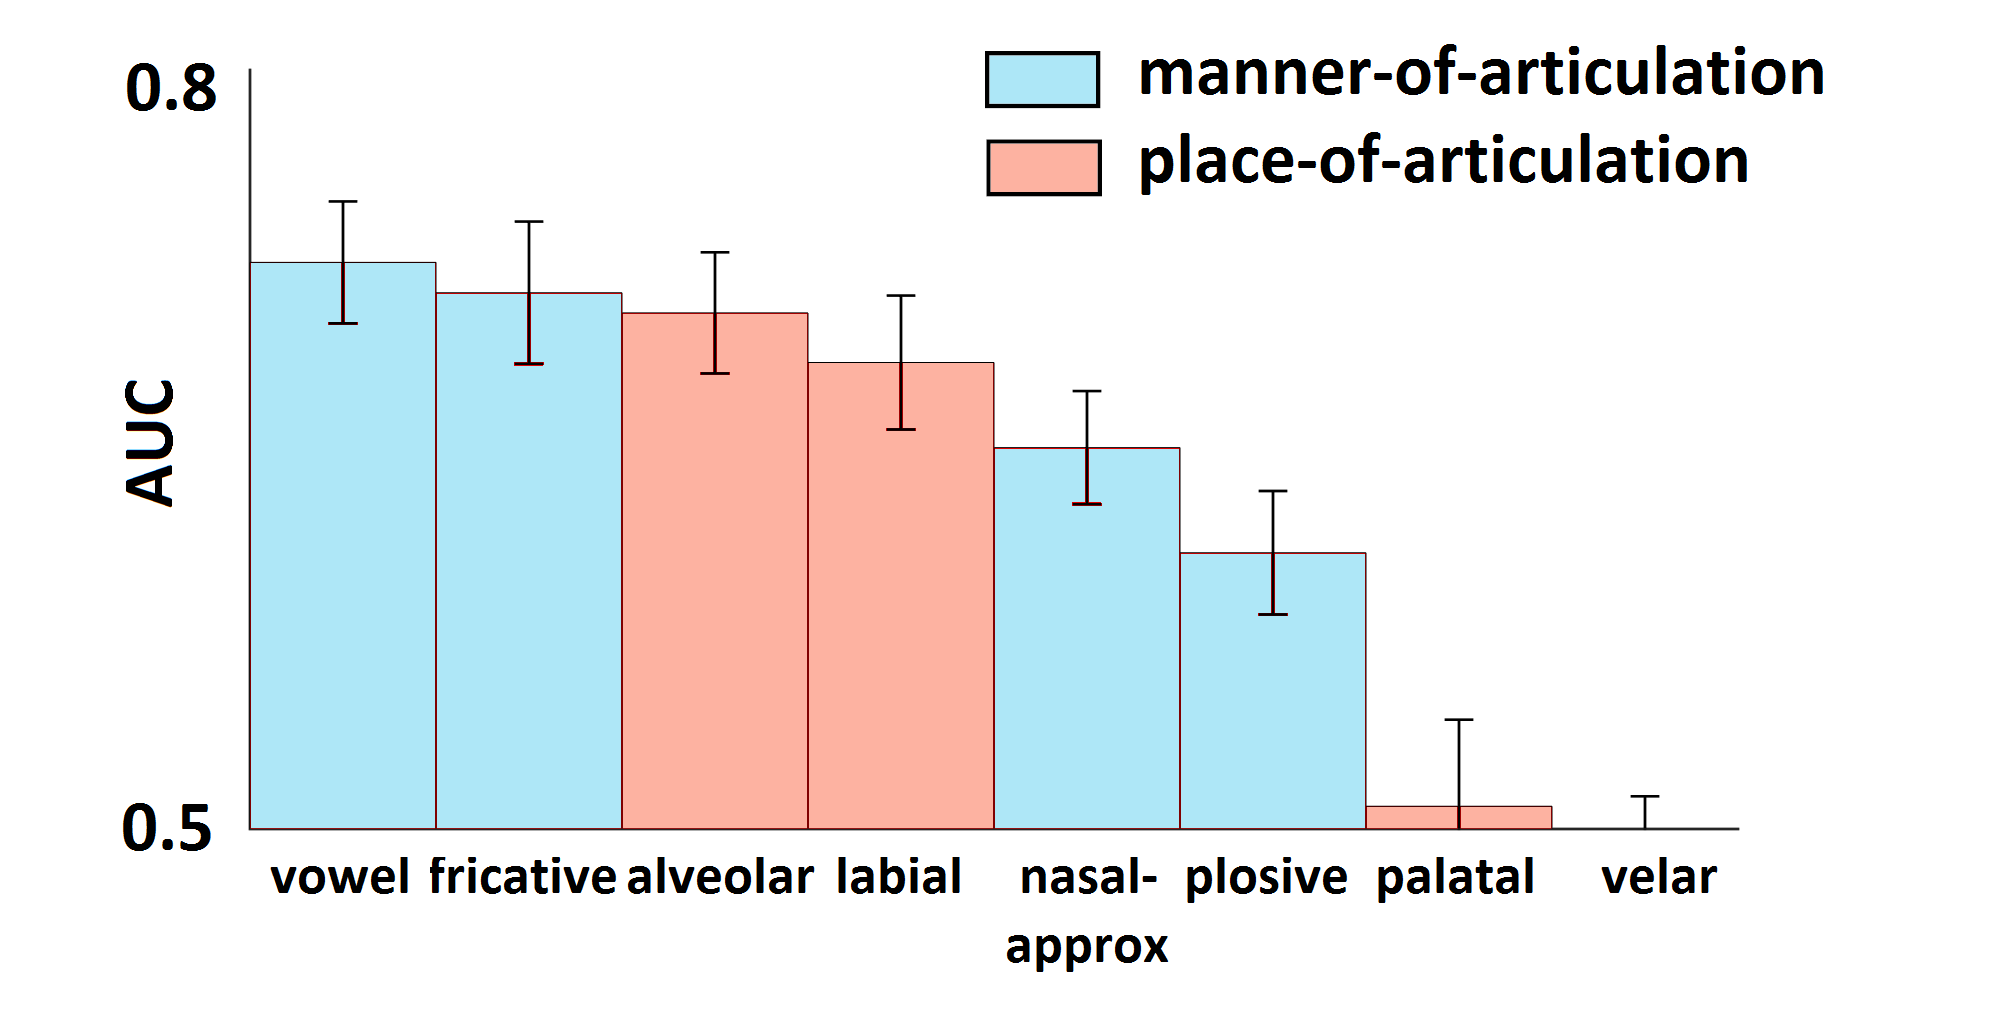
\includegraphics[width=\linewidth]{Figures/Ch3/Figure5_new.png}
\caption{AUC values for each binary feature, e.g., [+nasal] vs. [-nasal], [+labial] vs. [-labial]. AUC values were determined from the posterior probabilities of the Na\"{i}ve-Bayes model and phoneme identities of the test samples; Error-bars are calculated across test sets (see text, section 3.2.2).}
\end{figure}

\subsection{A comparison between neural and behavioral data}
Perceptual phoneme similarity in the cognitive system can be estimated from behavioral tasks, assuming the more confusable two phonemes are the more similar they are \citep{Tversky1977, Shepard1987}. We test whether phoneme similarity, as estimated from behavioral tasks, is reflected in neural activity in the STG during listening to the same set of phoneme stimuli. For this, we generate two phoneme-similarity matrices - a behavioral and a neural one. Behavioral similarity is derived from confusion errors made by human subjects, and neural similarity is derived from the representations of the STG responses (see Methods section 3.3.2 and 3.3.4). We evaluate the relation between the cognitive and neural functional organization, by calculating the Spearman correlation between the behavioral and neural similarity matrices. Results show a moderate correlation between the two ($\rho = 0.45, p-value < 10^{-3}$).

\section{Materials and methods}
\subsection{Patients and electrophysiological recording}
Data was collected from six patients with pharmacologically intractable epilepsy, implanted with intracranial depth electrodes to identify seizure focus for potential surgical treatment \citep{mukamel2012human}. Electrode location was based solely on clinical criteria. Each electrode terminated in a set of nine 40-$\mu$m platinum–iridium microwires \citep{fried1999cerebral} — eight active recording wires, referenced to the ninth. Signals from these microwires were recorded at 40 kHz using a 64-channel acquisition system. Before surgery each patient underwent placement of a stereotactic headframe, and then a detailed MR image was obtained using a spoiled-gradient sequence, followed by cerebral angiography. Both anatomical and angiography images were transmitted to a workstation in the operating room, and surgical planning was then performed, with selection of appropriate temporal and extra-temporal targets and appropriate trajectories based on clinical criteria. To verify electrode position, CT scans following electrode implantation were co-registered to the preoperative MRI using Vitrea® (Vital Images Inc.). The patients provided written informed consent to participate in the experiments. The study was approved by and conformed to the guidelines of the Medical Institutional Review Board at UCLA and the Tel-Aviv Sourasky Medical Center (Ichilov hospital).

\subsection{Stimuli and behavioral task}
Stimuli were constructed of either consonant-vowel (CV) pairs, or vowels /aeiou/ presented in isolation. The consonants in the CV syllables were according to the list in table 3.1, and the vowel was set to /a/ in order to reduce effects on the preceding consonant. To increase data size, we collected recordings from both Hebrew- and English-speaking patients. We therefore focused on a phoneme set that is approximately shared for both languages. Patients  were presented with 12 repetitions from each CV pair or vowel, 4 from each speaker, in a random order (ISI = 1 second). The patients were instructed to listen carefully to the syllables.


\begin{landscape}% Landscape page
\begin{table}
\centering % Center table
\tiny
\begin{tabular}{|c|c|c|c|c|c|c|c|c|c|c|c|c|c|c|c|c|c|c|c|c|c|c|c|c|c|}
\hline

&\multicolumn{21}{|c|}{Features}\\
\hline
&	a	&	e	&	o	&	i	&	u	&	n	&	m	&	l	&	j	&	f	&	v	&	s	&	z   & \textipa{S}	&	\textipa{Z}	&	p	&	b	&	t	&	d	&	k	&	g	\\
\hline

$sonorant$	&	+	&	+	&	+	&	+	&	+	&	+	&	+	&	+	&	+	&	-	&	-	&	-	&	-	&	-	&	-	&	-	&	-	&	-	&	-	&	-	&	-	\\
$vowel$	&	+	&	+	&	+	&	+	&	+	&	-	&	-	&	-	&	-	&	-	&	-	&	-	&	-	&	-	&	-	&	-	&	-	&	-	&	-	&	-	&	-	\\
$nasal$	&	-	&	-	&	-	&	-	&	-	&	+	&	+	&	-	&	-	&	-	&	-	&	-	&	-	&	-	&	-	&	-	&	-	&	-	&	-	&	-	&	-	\\
$approximant$	&	-	&	-	&	-	&	-	&	-	&	-	&	-	&	+	&	+	&	-	&	-	&	-	&	-	&	-	&	-	&	-	&	-	&	-	&	-	&	-	&	-	\\
$fricative$	&	-	&	-	&	-	&	-	&	-	&	-	&	-	&	-	&	-	&	+	&	+	&	+	&	+	&	+	&	+	&	-	&	-	&	-	&	-	&	-	&	-	\\
$plosive$	&	-	&	-	&	-	&	-	&	-	&	-	&	-	&	-	&	-	&	-	&	-	&	-	&	-	&	-	&	-	&	+	&	+	&	+	&	+	&	+	&	+	\\
labial	&	-	&	-	&	-	&	-	&	-	&	-	&	+	&	-	&	-	&	+	&	+	&	-	&	-	&	-	&	-	&	+	&	+	&	-	&	-	&	-	&	-	\\
coronal	&	-	&	-	&	-	&	-	&	-	&	-	&	-	&	+	&	-	&	-	&	-	&	+	&	+	&	+	&	+	&	-	&	-	&	+	&	+	&	-	&	-	\\
dorsal	&	-	&	-	&	-	&	-	&	-	&	-	&	-	&	-	&	+	&	-	&	-	&	-	&	-	&	-	&	-	&	-	&	-	&	-	&	-	&	+	&	+	\\
alveolar	&	-	&	-	&	-	&	-	&	-	&	+	&	-	&	+	&	-	&	-	&	-	&	+	&	+	&	-	&	-	&	-	&	-	&	+	&	+	&	-	&	-	\\
palatal	&	-	&	-	&	-	&	-	&	-	&	-	&	-	&	-	&	+	&	-	&	-	&	-	&	-	&	+	&	+	&	-	&	-	&	-	&	-	&	-	&	-	\\
velar	&	-	&	-	&	-	&	-	&	-	&	-	&	-	&	-	&	-	&	-	&	-	&	-	&	-	&	-	&	-	&	-	&	-	&	-	&	-	&	+	&	+	\\
\hline

\end{tabular}
\captionsetup{justification=centering}
\caption{List of consonant and vowels in the experiment}
\end{table}
\end{landscape}

All stimuli were recorded in an anechoic chamber with a RØDE NT2-A microphone and a Metric Halo MIO2882 audio interface, at a sampling rate of 44.1kHz. Stimuli were generated by two male and one female Hebrew speakers. The total number of stimuli was 63 (21 phonemes * 3 speakers). Length and pitch (by semi-tone intervals) were compared across recorded tokens to choose the most highly comparable stimulus-types. This was done by looking at differences in timeline arrangement, using built-in pitch tracker in a commercial software (\textit{Logic Pro X}). Further cleaning of noise residues in high resolution mode was done using \textit{Waves X-Noise} software. Figure 3.6 shows an example of the waveform of the syllable /\textipa{S}a/ (top), with the corresponding spectrogram (bottom), articulated by one of the male speakers. 

\begin{figure}[h]
\vspace{.3in}
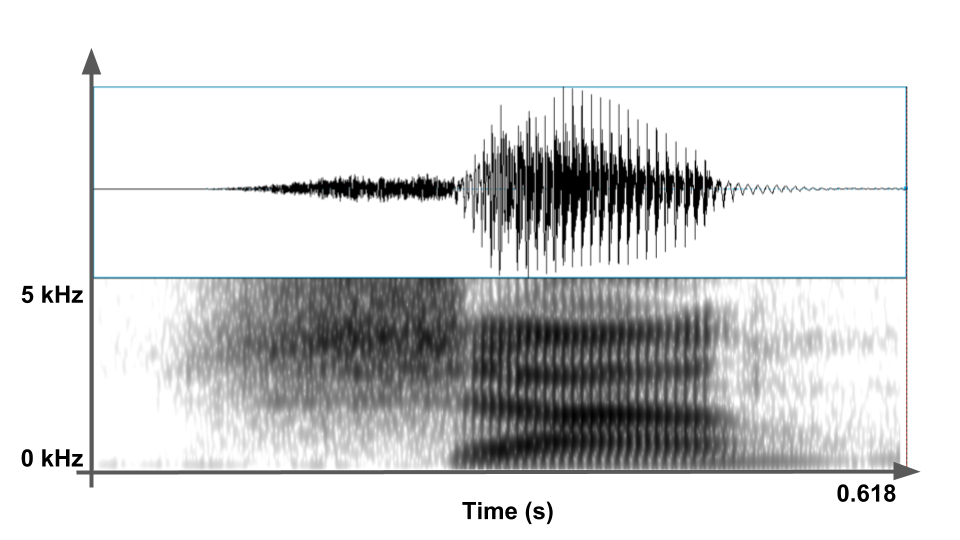
\includegraphics[width=\linewidth]{Figures/Ch3/spectrogram_sha.png}
\caption{An example of the waveform (top) and the corresponding spectrogram (bottom) of the phoneme /\textipa{S}a/, articulated by one of the male speakers.}
\end{figure}

\subsection{Data preprocessing}
To detect spiking activity, the data was band-pass filtered offline between 300 and 3000 Hz and spike sorting was performed using WaveClus \citep{quiroga2004unsupervised}, similar to previous publications \citep{quiroga2005invariant}. This process yields for each detected neuron a vector of time stamps (1 ms resolution) during which spikes occurred. To assess responsiveness of each neuron to the phonemes we compared speech to non-speech response. For this, we computed a t-test between the spike-count distribution before stimulus onset (-500-0ms) and after (0-500ms). Neurons with statistically-significant responses ($p-value<0.05$) were included in subsequent analyses. 

\subsection{A comparison between neural and behavioral data}
To test whether phonemes similarity at the behavioral level corresponds with population spiking activity in single STG neurons, we estimate two phoneme-similarity matrices - a behavioral and a neural one. The former is calculated from phoneme confusability according to: $S_{ij}=\frac{p_{ij}+p_{ji}}{p_{ii}+p_{jj}}$, where $p_{ij}$ is the probability of confusing phoneme $i$ with phoneme $j$ (section 2.2.2). The latter is based on neural activity in the following way: first, we calculated the standard score (z-score) of the spike-count activity in the optimal integration window. Next, for each pair of phonemes $i$ and $j$, we calculated the Euclidean distance $d_{ij}$ \citep{khalighinejad2017dynamic}, and then the phoneme similarity according to the following (monotonic) function: $S_{ij}=exp(-d_{ij})$. Finally, we performed Spearman rank correlation between the two matrices. The result is therefore not affected by the exact shape of the function. 

\section{Summary and discussion}
We recorded neural activity from six patients during a listening task in which vowels and consonant-vowel syllables were aurally presented. We characterized spiking activity from fourteen neurons in the STG that were consistently responsive to the speech stimuli. We inquired into three research questions: (1) we examined whether the neural representations of phoneme stimuli, based on single-cell activity, are local or distributed; (2) We tested whether the organization of neural representations of phonemes at the cellular level is dominated by manner or by the place-of-articulation dimension; Finally, (3) we examined the extent to which cognitive representations of phoneme perception match with neural representation extracted from single-cell activity in the STG during a listening task.

The first result of this study shows that phoneme representations of STG cells recorded in the experiment, are rather distributed, with mean sparseness \citep{treves1991determines} of $\bar{a}=0.59$, and only few units selective to a small set of phonemes (figure 3.3). Previous studies have found rather sparse representations in the auditory cortex of unanesthetized rat \citep{hromadka2008sparse}, or in the human STG using other measures to estimate population sparseness \citep{chan2013speech}. However, \citet{rolls1995sparseness} found similar sparseness values for temporal cortical neurons of primates in response to face stimuli, suggesting that the similarity among their stimuli might be the cause for the relatively high sparseness values found, as can be the case here. We note that despite the relatively high sparseness values of the units found in this study, it is possible that the population activity in response to phoneme stimuli is sparse \citep{olshausen2004sparse}. Due to the small number of units in each subject, this study cannot well estimate the population sparseness.

Next, we characterized the seemingly distributed, yet possibly clustered, response patterns to different phonemes, in several ways. First, we represented each phoneme in activity space in which dimensions correspond to estimated firing-rates, calculated in time bins of the most informative time window found for each unit. We then visualized the structure of phoneme representations by projecting it into a lower dimensional space. The resulting structure reveals a separate representation of sonorant and obstruent phonemes, as was previously shown in ECoG studies \citep{Mesgarani2014}. The sonorant-obstruent distinction can be described with acoustic properties but not with motor properties, as sonoarnts have a clear acoustic marker of resonance, with regular patterns in their waveform, whereas sonorant and obstruent involve varied articulations.

To further specify relations among phoneme representations, we next examined the hierarchical clustering of the data in activation space. We found that most of the sonorant and obstruent phonemes cluster separately, and that strident fricatives form a sub-cluster of the obstruent one. These results further point to a functional organization based on acoustic cues. First, as mentioned, sonorants are highly resonant and have identifiable formant structure compared to obstruents. Second, stridents have a clear acoustic footprint, characterized by high intensity and high-frequency energy. 

To further quantify this, we trained a probabilistic classifier, which mimics the generation process of spikes, as recorded by the units. We then compared model predictions when grouping phonemes according to various phonological features. Panels C and D of figure 3.4 present the resulting confusion matrices. It is observed that the confusion matrix of manner features is more diagonal compared to place-of-articulation features. Similarly, figure 3.5 presents AUC values for binary classifications for the same set of features, resulting with all four manner features significantly above chance level ($p-value<0.001$), whereas for place-of-articulation only two features are above random guess ($AUC = 0.5$). Taken together, it adds to previous results, suggesting that neural representations in the STG are dominantly organized by the manner-of-articulation dimension, thus providing additional support to auditory theories of speech perception. 

Finally, we compared the neural and cognitive organizations of phonemes, as estimated from single-cells activity and behavioral data, respectively. We found that spiking activity from the fourteen selected neurons reflects phoneme similarities derived from behavioral results, based on phoneme-confusion experiments using the same set of stimuli (section 2.3.3). Specifically, the nasal and approximant features show a distinct neural representation with respect to other feature classes, which corresponds to their relatively high perceptual saliency, as described in chapter 2.

Speech signals are composed of continuous streams of high-dimensional acoustic information, which must be encoded in the auditory pathway in a way that ensures robust categorization. The auditory pathway shows an increasing encoding specificity and invariance for speech sounds, from relatively simple acoustic features in early stages, to complex spectrotemporal acoustic patterns in cortical regions. In humans, invariance to phonetic features is thought to be found outside the primary auditory cortex, in STG and STS subregions \citep{Dewitt2012} (in animals, \citealp[see]{mesgarani2008phoneme}). This study provides another layer of evidence, showing that the functional organization of phonemes in the STG, as revealed by population spiking activity, is in accordance with auditory theories \citep{stevens1989quantal, stevens2002toward}, and in contrast to motor theories of speech perception \citep{liberman1985motor, browman1992articulatory}.